\chapter{A Brief History of the Primeiro Comando da Capital}
\label{ch:chap3}

%----------------------------------------------------------------------------------------

\begin{chapquote}{Dialogue between a detainee and a prison officer in S\~{a}o Paulo, quoted in Karina Biondi, \textit{Junto e Misturado}\footnote{Original dialogue in Portuguese: ``-- [\dots] Funcion\'{a}rio \'{e} funcion\'{a}rio, ladr\~{a}o \'{e} ladr\~{a}o. Eu n\~{a}o dei essa liberdade pro senhor. Numa dessas a\'{i}, os caras podem interpretar errado a\'{i} minha pessoa e eu posso passar por safado na cadeia.\\
-- Isso n\~{a}o tem nada a ver.\\
-- N\~{a}o tem nada a ver pro senhor, mas na cadeia o barato \'{e} louco. Respeito \'{e} bom e eu admiro, mas se n\~{a}o tiver um respeito da parte do senhor, a\'{i} a gente vai ter que correr atr\'{a}s das provid\^{e}ncias.'' \citep[84]{biondi2010junto}}.}
-- [\dots] An officer is an officer, a thief is a thief. I didn't give you this freedom, Sir. If things go like that, the guys will get me wrong and I can be taken as a snitch in prison.\\
-- It's not like that.\\
-- It's not like that to you, Sir, but in jail things are crazy. Respect is good and I admire that, but if there's no respect from your side, Sir, then we'll have to take action.
\end{chapquote}

Historical reasoning is never neutral. Describing historical events is knowingly a partial, conflicting enterprise. As pointed out by \citet[401]{istiaisyah2001textual}, historical accounts are ``[\dots] rendered ideological by the very act of being conveyed in a narrative form, for language is both the purveyor of meaning and the principle locus of ideology'' \citep[401]{istiaisyah2001textual}. Similarly, \citet[1]{thompson2000voice}, the British oral historian, once argued that ``all history depends ultimately upon its social purpose'', and there is no reason to believe that a history of prisoners would be different. While there is a certain degree of consensus about what structural causes allowed the PCC to emerge \citep[]{adorno1991sistema, cruz2013recent, redigolo2012sistema, salla2007montoro}, the history behind the organisation's true origins is still contested and probably instrumentalised by different actors. In this chapter, I adopt one of several accounts of the emergence of the PCC in S\~{a}o Paulo. I present here the version which is usually told by the prisoners themselves, and has been reported by most of the recent literature on the gang \citep[]{amorim2003cv, biondi2010junto, dias2011pulverizaccao, jozino2004cobras, souza2007pcc}. Unfortunately, there is no way of assessing the veracity of every detail in that narrative. On the one hand, prisoners either do not know or do not remember the chain of events that resulted in the rise of the PCC; on the other hand, many of them simply prefer not to say something that confronts the story told by the gang for understandable motives. Therefore, what I describe here is something close to an ``official history'' of the \textit{Comando}, starting from its origins in the wake of the killing of 103 prisoners in S\~{a}o Paulo's largest prison to the present day. Firstly, I begin with a brief contextualisation of the state of the penal system in S\~{a}o Paulo in the 1980s. Then, I adopt the chronology suggested by \citet{dias2011pulverizaccao} and divide the PCC's history in three parts, namely foundation, expansion, and consolidation.

\section{Failed Hopes: From Democratisation to the Carandiru Massacre}

From 1964 to 1985, Brazil was governed by members of the Armed Forces. A military junta headed by the Army Chief of Staff, Marshal Humberto de Alencar Castelo Branco, ousted the leftist President Jo\~{a}o Goulart on 31st March 1964, and only returned the political power to a civilian leadership more than two decades later \citep[]{skidmore1988politics}. The coup d'\'{e}tat was initially presented as a short-lived measure against corruption and communism. In the words of Ernesto Geisel (Army General, President from 1974 to 1979), the coup's main goal was  ``[\dots] to correct, not to build something new'' \citep[apud][138]{gaspari2002envergonhada}. Nevertheless, after the \textit{linha dura}\footnote{Literally, ``hardliners''. The recent historiography notes that in 1967 there was a sort of ``coup within the coup'' \citep[]{gaspari2002escancarada}, where nationalistic groups within the Army managed to remove the moderate officials from their positions and increased the repression against civilians in order to ``deepen the revolution'' \citep[33-39]{fico2004versoes}.} successfully manoeuvred to take the presidency in 1967, a speedy return to democracy seemed unlikely. Although the Armed Forces tried to keep a democratic fa\c{c}ade over the whole period\footnote{Regular elections were held during most of the military regime, even though the government often changed election rules in its favour and several important positions in the country were not open for political competition. An opposition party, the \textit{Movimento Democr\'{a}tico Brasileiro} (Brazilian Democratic Movement -- MDB), was allowed to participate in elections. The party had considerable success after 1974 \citep[]{kinzo1988oposiccao} and currently is one the country's most important political forces \citep[]{demelo2001pmdb}. Furthermore, the Armed Forces tried to avoid a personal dictatorship in the Brazil, thus all four presidents had a clearly determined term and this rule was always taken seriously \citep[]{alves2014state}. Despite this democratic cover, the regime curtailed freedom of speech and of the press \citep[]{smith1997forced}, and also systematically used torture against dissidents and protesters \citep[]{arns1985brasil, coimbra2001tortura, zirker1988democracy}.}, physical coercion was widely employed as a means to maintain the stability of the regime. In this regard, the police was a key institution to the government. In a division that lasts until the present day, the dictatorship created two types of police in Brazil: the \textit{pol\'{i}cia civil} (civilian police), mainly responsible for investigations, and the \textit{pol\'{i}cia militar} (military police), responsible for public order and notably more repressive than its civilian counterpart. As described by \citet[91]{bicudo2000unificaccao}, this dual policing model was ``[\dots] built in the years of the military dictatorship to protect the state, and it follows the ideas expressed by the Doctrine of National Security\footnote{This doctrine was formulated in 1958 by the General Golbery do Couto e Silva and turned into law 10 years later, after the hardliners controled the federal government. It posited that the main threat to the Latin America's national security was the ``enemy within'', local communist groups that became powerful after the Cuban Revolution (1958). Therefore, every country in the region should quickly identify and repress left-wing groups \citep[]{fernandes2009reformulaccao}.}, which declared that whoever is not a friend is an enemy and should therefore be treated as such. This line of action qualified, during that period of our [Brazilian] history, the actions of the police''.

This legacy of police violence in Brazil did not end with the return to democracy. In the 1980s, the situation in prisons was as bad as it used to be during the authoritarian regime. However, a few state governors tried to ameliorate living conditions for prisoners and change the draconian penal system which had been in place in the military rule. In S\~{a}o Paulo, governor Andr\'{e} Franco Montoro\footnote{Montoro's term lasted from 1983 to 1987. He was elected as a member of the MDB, the main opposition (democratic) party.} and his Secretary of Justice Jos\'{e} Carlos Dias adopted a new approach to manage state prisons. The main ideas behind their ``prison humanisation policy'' were to create mechanisms of dialogue between inmates and prison agents, hire better-trained professionals to the penitentiaries, and reorganise the penal system so that it could achieve its primary goal, the future socialisation of the detainee \citep[75]{salla2007montoro}. 

One of the most important innovations of that period was the institutionalisation of the \textit{Comiss\~{o}es de Solidariedade} (``Solidarity Commissions'') \citep[]{alvarez2013comissoes}. The commissions were composed by groups of prisoners -- elected via secret ballots by the inmates themselves -- and its purpose was to provide a direct channel of communication between inmates and the Secretary of Justice. In practice, the commissions first addressed questions concerning jail time and police abuse. However, two factors soon delegitimised the commissions. First, the series of rebellions that took place in state prisons in mid-1985 (at the Casa de Deten\c{c}\~{a}o de S\~{a}o Paulo and Araraquara Penitenciary) and in September 1986 (at the Presidente Venceslau Penitentiary). Second, a rumour about the supposed existence of the \textit{Serpentes Negras} (``Black Serpents''), a group of violent prisoners who aspired to control the commissions and use it to punish other detainees \citep[72]{alvarez2013comissoes}. Although it was never proven that such a group actually existed, the rumour was strong enough to cause a stir in the local media, and it eventually galvanised the public opinion against Montoro's ``lenient'' penal policies \citep[]{paixao1987recuperar}. Additionally, since many penitentiary directors and prison staff did not agree with the governor's ``humanisation policies'', their mounting resistance forced the governor to abandon the project \citep[]{teixeira2009prisoes}. 

The next two governors of S\~{a}o Paulo, Orestes Qu\'{e}rcia (1987--1990) and Luiz Ant\^{o}nio Fleury (1991--1994), adopted an openly conservative stance against the inmate population. In Qu\'{e}rcia's four-year term, the number of prisoners increased from 14,988 to 23,516, and the number of facilities grew from 21 to 37 across the state  \citep[77]{salla2007montoro}. Fleury's term was the apex of the repression against prisoners in S\~{a}o Paulo: the aforementioned Carandiru Massacre. On 2nd October 1992, a prisoners' revolt in the Casa de Deten\c{c}\~{a}o\footnote{As mentioned in \autoref{ch:chap2}, the prison was also known as the Carandiru Penitentiary due to the neighbourhood in which it was located. Inmates called it \textit{Casar\~{a}o} (``The Big House'').} triggered a disproportional retaliation by the police forces and 103 unarmed inmates were executed inside prison cells \citep[]{adorno2007organized, pieta1993pavilhao}. Hosting more than 7,000 prisoners -- the official capacity was 3,250 -- Carandiru was the largest penitentiary in South America, and the massacre remains the most serious human rights violation in Brazil after the democratic transition \citep[]{ahnen2003between}.

The massacre was also remarkable for another reason. According to several sources \citep{amorim2003cv, biondi2010junto, dias2011pulverizaccao, jozino2004cobras, souza2007pcc}, the PCC was founded as a response to that event, and its members claim that one of the main purposes of the organisation is to prevent another police abuse. The Carandiru massacre, therefore, marks the beginning of a new era in the penal system in S\~{a}o Paulo, where inmates began to organise themselves into a single, large group that could not only offer resistance to authority abuse, but also prevent violence amongst the incarcerated population. The prison system had entered a new phase.

\begin{center}
\begin{figure}[bth]
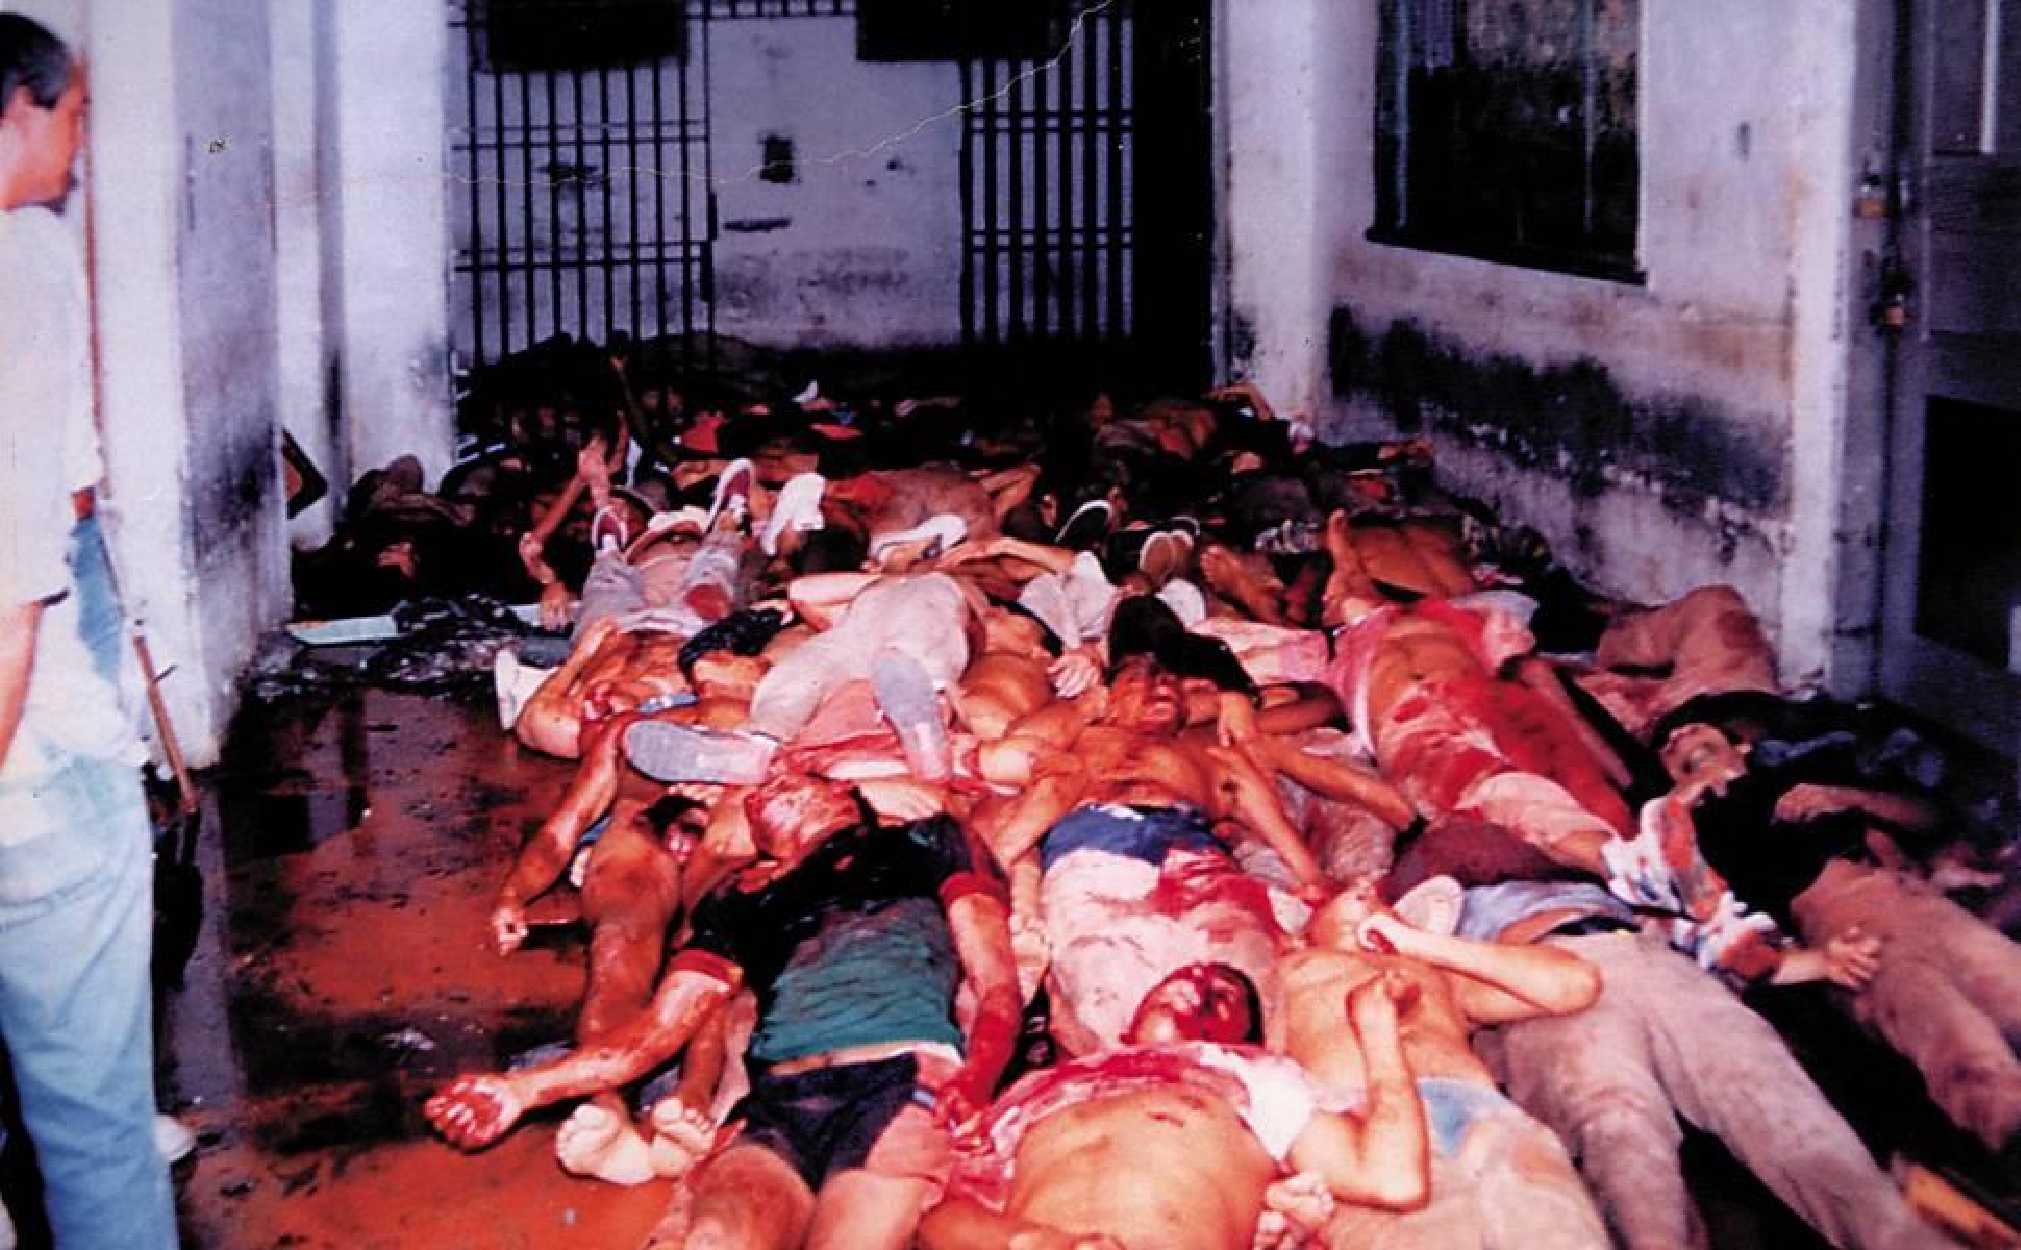
\includegraphics[height = 8cm, width = 1\linewidth]{gfx/fig4}
\caption[Inmates killed by the police in the Carandiru Massacre, 1992]{Inmates killed by the police in the Carandiru Massacre\footnotemark}
\label{fig:fig4}
\end{figure}
\end{center}

\footnotetext{Source: Folha de S\~{a}o Paulo.}

\section{Foundation: After Carandiru}

The Primeiro Comando da Capital was officially founded on 31st August, 1993, by eight detainees\footnote{Namely, Mizael Aparecido da Silva (``Miza''), Wander Eduardo Ferreira (``Cara Gorda'' -- ``Fat Face''), Ant\^{o}nio Carlos Roberto da Paix\~{a}o (``Paix\~{a}o''), Isa\'{i}as Moreira do Nascimento (``Esquisito''  -- ``Weirdo''), Ademar dos Santos (``Da F\'{e}'' -- ``Faith''), Ant\^{o}nio Carlos dos Santos (``Bicho Feio'' -- ``Ugly Beast''), C\'{e}sar Augusto Roris da Silva (``Cesinha'' -- ``Little C\'{e}sar'') and Jos\'{e} M\'{a}rcio Fel\'{i}cio (``Gelei\~{a}o'' -- ``Big Jelly'') \citep[]{folha2006criada}. The inmates are mainly known by their nicknames. \citet[69]{biondi2010junto} notes that there are different versions for the foundation of the PCC, but apparently the prisoners abandoned all of them in favour of the story told by \citet[]{jozino2004cobras}, who published a widely-circulated book in the mid-2000s. \citet[69]{biondi2010junto} also writes that it was not the first time she saw such examples of ``collective amnesia'', when PCC members seem to ``forget'' or downplay certain facts that may cause rife between prisoners.} of the \textit{Casa de Cust\'{o}dia de Taubat\'{e}} (``Taubat\'{e} Custody House''). The jail is located in the countryside of S\~{a}o Paulo \citep[60]{matos2009lado}, and was then considered the safest penitentiary in the state. Nevertheless, as described by William Langewiesche \citep[]{vanityfair2007pcc}, 

\begin{quotation}
Conditions there were atrocious. The prisoners lived locked alone into 160 dark and putrid cells, surviving on filthy slops, defecating into holes they could not flush, and subject to beatings by the guards. They were released into the yards only every few days, and in groups of merely five. Some committed suicide. Most, however, were tough, and managed not only to remain vital, but also to communicate fully from cell to cell.
\end{quotation}

A discussion that allegedly began after a football match was the trigger of a serious fight between inmates. Two prisoners were killed and others were wounded\footnote{The story goes that Gelei\~{a}o broke the neck of a rival gangster on the pitch, in front of all criminals and guards \citep[134]{santos2010dimensao}.}. The eight remaining detainees, fearing a brutal punishment by the warden, decided to swear a public vow of mutual defence. The gang was christened as \textit{Primeiro Comando da Capital}, and is also referred to as \textit{Partido do Crime} (``Criminal Party''), \textit{Fam\'{i}lia} (``Family''), \textit{Quinze} (``Fifteen''), and \textit{15.3.3} (``PCC'' in the Brazilian alphabet) \citep[25]{biondi2010junto}. The group soon published their statute, probably written by Miza. Their constitution, only 16 articles long, lays out the rules members are expected to obey. The statute commands:

\begin{enumerate}
\item Loyalty, respect and solidarity to the Party, above all.
\item The Struggle for liberty, justice and peace.
\item The unity of the Struggle against injustice and oppression inside prisons.
\item The contribution from those who are in liberty to the brothers inside prisons through lawyers, money, help to family members and prison outbreak operations.
\item The respect and solidarity to all members of the Party, so there are no internal conflicts, for he who causes conflicts within the Party, trying to divide the brotherhood will be excluded and shunned from the Party.
\item Never use the Party to solve personal conflicts with outsiders. Because the ideals of the party are above personal conflicts. But the party will always be loyal and supportive to all its members so that they do not suffer any inequality or injustice in external conflicts.
\item He who is in liberty and enjoying a good life, but forgets to contribute to the brothers in jail, will be condemned to death without forgiveness.
\item Members of the Party have to set an example, and for that reason the Party does not allow mugging, rape and extortion within the System.
\item The Party will not tolerate lies, treason, jealousy, greed, misdirection, selfishness and personal interest. It values truth, fidelity, manhood, solidarity and the interest in the common good, because we are one for all and all for one.
\item Every member has to respect the order and discipline of the Party. Each one will be paid accordingly to what he deserves for what he has done. Everyone's opinion will be heard and respected, but the final decision will be made by the founders of the Party.
\item The Primeiro Comando da Capital (PCC) was founded in the year of 1993, in an overwhelming and tireless struggle against oppression and injustice in the concentration camp of the Casa de Cust\'{o}dia (``House of Custody'') of Taubat\'{e}, with the absolute motto ``Liberty, Justice, and Peace''.
\item The Party will not tolerate internal rivalries, disputes for the leadership of the Command, as each member of the Command knows his own role according to his own capability to execute it.
\item We must remain united and organised to avoid a similar or worse massacre as the one which occurred on 2nd October, 1992, when 111 prisoners were cowardly murdered, a massacre that will never be forgotten in the consciousness of the Brazilian society [the Carandiru Massacre]. For we from the Command will change prison practices [that are], inhumane, full of injustices, oppressive, [with] torture and prison massacres.
\item The priority of the Command is to put pressure on the State Government to deactivate the Concentration Camp of House of Custody of Taubat\'{e}, from where the roots of the Command originated, in the middle of such inglorious and atrocious suffering.
\item Emanating from the Central Command of the Capital of the HQ of the State, the simultaneous action directives in all of the State's prison facilities, in a truceless, borderless war until the final victory.
\item The most important of all is that no one will stop us in this struggle, for the seed of the Command has spread to all prison systems of the state and we have managed to structure ourselves outside [of prisons] as well, with many sacrifices and irreparable losses, but we have consolidated ourselves at the state level and in the middle and long run we will consolidate ourselves at the national level. In an alliance with Comando Vermelho (CV) and PCC, we shall revolutionise the country from within prisons and our armed wing will be the terror of the powerful oppressors and tyrants that used the Taubat\'{e} Annex and Bang\'{u} I in Rio de Janeiro as an instrument of vengeance from the society to the creation of monsters.

\vspace{.3cm}

We know our strength and the strength of our Powerful enemies, but we are ready and united, and a united people will never be defeated.

\vspace{.3cm}

LIBERTY! JUSTICE! AND PEACE!

\vspace{.3cm}

PCC Headquarters, First Command of the Capital, in alliance with Comando Vermelho (CV)

\vspace{.3cm}

UNITED WE SHALL WIN!\footnote{The statute was first publish by \citet{folha2001estatutopcc}. Capital letters in the original. To the best of my knowledge, the statute has never been changed or amended.}
\end{enumerate}

The PCC statute performs the three functions of criminal constitutions described by \citet[]{leeson2010criminal}. First, the statute promotes consensus among PCC members by creating common knowledge about what the organisation expects from them and what they can expect of each other. All articles, in this sense, have such function. Second, it also regulates behaviour that, while beneficial to private individuals, may be damaging to the PCC as a group. The fact that criminals cannot invoke the gang to solve personal issues, for instance, is a clear example of that. Whereas the PCC may indeed be used as a mediation tool within and outside prisons \citep[]{dias2009ocupando}, the Command cannot be called to address questions which are \textit{strictly personal}, like a family feud. Finally, the statute mentions what are the punishments for deviations to the expected behaviour individuals are supposed to have after they become members of the cartel. Prisoners who try to ``divide  the  brotherhood'' will be banned from the group and, curiously, those do not finance the gang shall be put to death. Such harsh punishment probably indicates that the organisation has been concerned with expanding his reach since its foundation, what makes collaboration one of the most important tasks for the group members.

%The manner by which individuals join to the gang goes as follows. After being \textit{batizados} (``baptised'') by the cartel\footnote{The baptism usually works like this: an inmate who is already in a PCC-dominated prison (called \textit{primo} -- ``cousin'') can become a full member of the PCC after being formally invited to join the gang by two other \textit{irm\~{a}os} (``brothers''), detainees who are already affiliated with the cartel. If the inmate decides to accept the offer, those two detainees who invited him will be then considered his \textit{padrinhos} (``godfathers'') and take responsibility for future actions of their proteg\'{e}e. Since the process implies costs for the two detainees, they tend to indicate an third inmate only after long periods of friendship. This explains why prisoners may stay as \textit{primos} for years before they are officially accepted in the PCC \citep[210]{biondi2007relacoes}.}, the inmates are called \textit{irm\~{a}os} (``brothers'') and can claim that they belong to the group. Criminals generally address each other as \textit{ladr\~{a}o} (``thief'') regardless of the crime perpetrated by the individual, and although PCC members also use \textit{irm\~{a}os} to refer to each other, the more general term ``thief'' is employed very often. Its meaning, if derogatory, neutral or even complimentary, depends widely on context \citep[]{marques2009crime}. In contrast, police officers, members of rival gangs, and other enemies are called \textit{coisa} (``thing'') or \textit{verme} (``worm'') \citep[169]{dias2011pulverizaccao}. 

%There are three ``political positions'' that a PCC member can occupy, namely \textit{faxinas} (``cleaners''), \textit{pilotos} (``pilots''), and \textit{torres} (``towers'') \citep[110-123]{biondi2010junto}. The first group comprises inmates who work as mediators between prisoners and state institutions, and are also in charge of the cleaning and management of everyday affairs. \textit{Pilotos} are ``spokespeople'' to the inmates, and are democratically elected by the detainees to voice their concerns and represent them in negotiations \citep[1102]{dullo2012biondi}. ``Pilots'' are elected at many different levels, being usually a representatives of the cell, corridor and prison. The role of the \textit{torres} is a bit more difficult to grasp. From what is currently known, the towers are groups of senior inmates who jointly debate and decide (usually by consensus) some of the most serious issues regarding the organisation, such as giving order, solving disputes and ordering punishments. However, PCC members are quite elusive about the meaning and scope of such groups, and so far there is not a single academic research that clarifies under what circunstances the torres are called to act and what tasks they are allowed to perform \citep{biondi2010junto}.

Drauzio Varella, a respected oncologist who served as a volunteer for 13 years at Carandiru\footnote{Varella also wrote a long memoir about inmate life in Carandiru \citep[]{varella1999estaccao}, a text with later became the main source for a successful drama film directed by Hector Babenco. See: \href{http://www.sonyclassics.com/carandiru/}{http://www.sonyclassics.com/carandiru/}. Access:  25th May, 2014.}, mentions how important it is for prisoners to organise themselves, and how effective that social division of labour used to be. In an interview to \citet[]{vanityfair2007pcc}, the doctor said:

\begin{quotation}
Rats who are overcrowded become violent. There have been experiments in the United States to show it. But Carandiru showed that people in those same conditions will organise, and establish rules for their survival. The rules in Carandiru evolved as the prison grew more crowded. They were not written down, but were passed on as understandings. For instance, you had to wash. Every day. And during meal delivery you could not stay in the hallways. For hygiene. Inside the cells, when people were eating, you could not use the toilet. You could not spit. You could not cough. You could not pick your teeth. [\dots] Some of the cell blocks had more than a thousand prisoners. Five, six guys per cell. [\dots] I was so impressed that it was possible in Carandiru for these men to organise in such a way. But, you know, anarchy does not endure in human affairs. And there is no empty space for power in prison.
\end{quotation}

Despite such a high level of organisation and several attempts to mobilise themselves against the public authorities, S\~{a}o Paulo state government used to vehemently deny the groups' own existance \citep[]{bbc2012pcc}. State officials frequently said that there was no such thing as a prison gang in S\~{a}o Paulo, even though a couple of journalists had already collected clear evidence that a criminal organisation had been operating in the penal system \citep[]{jozino2004cobras, souza2007pcc}. In 1996, F\'{a}tima Souza -- an investigative journalist of one the Brazil's main TV channels -- presented the first piece of news where the PCC was presented as an organisation. Unsurprisingly, the government's response quickly dismissed what the journalist had published. In the Souza's words (emphasis mine) \citep[]{obs2007pcc}:

\begin{quotation}
I made a robust piece of news, eight minutes, and we aired it on Band\footnote{Bandeirantes Network, a national broadcasting company based in S\~{a}o Paulo. See: \href{http://www.band.uol.com.br/tv/}{http://www.band.uol.com.br/tv/}. Access:  25th May, 2014.}. For the first time the word ``PCC'' appeared in the scene. The government denied it, obviously. The secretary of prison administration, [Jo\~{a}o] Benedito [de Azevedo] Marques, even spoke to Jovem Pan [radio station] saying I invented such story to gain more points at IBOPE\footnote{IBOPE is the \textit{Instituto Brasileiro de Opini\~{a}o P\'{u}blica e Estat\'{i}stica} (``Brazilian Institute of Public Opinion and Statistics''), a firm that conducts research on media, public opinion and voting intention. It is widely known in Brazil, and its name is often used as a synonym for audience ratings. See: \href{http://www.ibope.com.br/}{http://www.ibope.com.br/}. Access:  26th May, 2014.}, and that what I was talking about a \textit{fiction} not about a \textit{faction}. This made me very angry. My own colleagues were making fun of me: ``So, where is the PCC, are you making news up?'' At the time, the only colleague in the press who took it seriously and decided to know more about it was Josmar\footnote{Josmar Jozino, journalist for the \textit{Di\'{a}rio de S\~{a}o Paulo} (``S\~{a}o Paulo Daily''), author of an important book on PCC \citep[]{jozino2004cobras}.}, which knew how I used to work and that I was not making up a story.
\end{quotation}

For many years there was a strong self-censorship in the public and private media about the existence of the PCC. \citeauthor{jozino2004cobras} (\citeyear{jozino2004cobras}, 143 apud \citeauthor{biondi2010junto}, \citeyear{biondi2010junto}, 74) comments that the editors of the newspaper he used to work

\begin{quotation}
[\dots] banned the use of the acronym PCC, the number $15.3.3$ and the name ``Primeiro Comando da Capital''. The acronym was banned indefinitely from texts, titles, subtitles, headlines or first-page covers. The newspaper should only refer to the PCC as ``criminal faction that dominates the prisons in S\~{a}o Paulo'', or ``criminal group'', or even ``criminal organisation.'' This rule was also extended to the remaining newspapers, magazines and radio and TV networks of the same group, based in Rio de Janeiro\footnote{The \textit{Di\'{a}rio de S\~{a}o Paulo} belongs to the Globo Network, the largest media conglomerate in Latin America. The TV network is the most well-known in Brazil, and the second largest in the world (after the American Broadcasting Company). It presently reaches 99.5\% of the Brazilian population. Any ban adopted by such a large company would surely have a strong impact in the Brazilian public. See: \href{http://redeglobo.globo.com/Portal/institucional/foldereletronico/ingles/g_globo_brasil.html}{http://redeglobo.globo.com/Portal/institucional/foldereletronico/g\_globo\_brasil.html}. Access:  26th May, 2014.}. The acronym CV and ``Comando Vermelho'' was banned.
\end{quotation}

Nevertheless, this false feeling of security did not last for long. A few years after its foundation, the PCC would stage two spectacular series of rebellions in the state, briefly described in \autoref{ch:chap1}. Here I focus on how the PCC organised itself and managed to perform such violent acts.

\section{Consolidation: The Rebellions of 2001 and 2006}

In the end of the 1990s, the PCC progressively expanded their control to other prisons in S\~{a}o Paulo. Apart from the group's own actions, two structural factors collaborated to the growth of the PCC in state prisons \citep[]{adorno2007organized}. First, S\~{a}o Paulo saw a remarkable increase in incarceration rates in the 1990s and 2000s\footnote{See \autoref{fig:fig2}.}. As the total number of detainees went up, the demand for physical and property rights protection in prisons by the inmates also increased which favoured the emergence of a broker and mediator such as the PCC. Also, the precarious conditions of the state jails forced the inmates to develop new ways of coping with scarcity. Thus, having a group which has already devised a set of rules that prisoners can follow in order to maintain order is something of great importance. Second, in an attempt to reduce their influence, several PCC leaderships were transferred to prisons in the countryside, sometimes very far from the capital. Nevertheless, against the government's expectations, instead of isolating the PCC members, the mobsters ended up establishing contact with local criminals, what soon enlarged the \textit{Comando}'s presence in other regions of the state \citep[103]{dias2011pulverizaccao}. 

The rise of the PCC was welcomed by the vast majority of inmates. Anecdotal evidence suggests that S\~{a}o Paulo's prison hierarchies were established mainly through the use of force, and all sorts of conflicts were solved either via physical punishment or by imposing strong humiliations to the individuals \citep[]{adorno1991sistema, ramalho1979mundo}. \citet[4]{negrini2002enjaulado}, himself a detainee in Carandiru prison, shows how common the confrontatios were. In his words,

\begin{quotation}
The scene that unfolded was common. The guards would only interfere after someone was on the floor, stabbed and bleeding. The remaining prisoners formed a large circle, also without interfering. Someone would only leave that [duel] dead or injured and completely demoralised. [\dots] As a result of these fights, prisoners will be respected [and treated] as strong and brave, as leader of their cells, as untouchables. 
\end{quotation}

Acts of violence seemed to be widespread in the penal system, and narratives of fights and physical disputes abounded in the specialised literature on S\~{a}o Paulo's state prisons. But even though physic strength did matter in prisons \citep[]{thompson1980questao, ramalho1979mundo}, there were always exceptions to the rule. Instead of being merely a crude, raw version of Thrasymachus' sentence in Plato's \textit{Republic} -- that ``[\dots] the just is nothing else than the advantage of the stronger''\footnote{See: \href{http://www.perseus.tufts.edu/hopper/text?doc=urn:cts:greekLit:tlg0059.tlg030.perseus-eng1:1.338c}{http://www.perseus.tufts.edu/hopper/text?doc=urn:cts:greekLit:tlg0059.tlg030.perseus-eng1:1.338c}. Access: 28th May, 2014.} (1.338c) -- Brazilian prisons were probably more similiar to the Hobbesian state of nature, where skills and tactics were crucial to survival. Hobbes' famous argument posits that ``[\dots] the weakest has strength enough to kill the strongest, either by secret machination or by confederacy with others that are in the same danger with himself'' \citep[61]{hobbes1985leviathan}. Drauzio Varella confirms Hobbes' insight and affirms that ``[\dots] strength had no role at Carandiru, because people had to sleep. And if you gather 20 guys, even Mike Tyson wouldn't stand a chance'' \citep[]{vanityfair2007pcc}. Since the possibility of temporarily ganging up with other prisoners was always present in jails, the lack of security was pervasive in Brazilian prisons. It affects the weak and the strong alike.

After the PCC started to control the prison system, many inmates claimed that the former chaotic environment was gradually replaced by a sort of \textit{pax mafiosa}, where disputes were solved through PCC tribunals and the use to violence was progressively limited. Commenting on the \textit{Party}, Aldair, an evangelical pastor interviewed by Sacramento \citep[apud][71]{biondi2010junto} told that:

\begin{quotation}
I am not defending crime, but before PCC's existence, prisoners used to suffer very much. They used to suffer because they belonged to different gangs. There used to be much extortion, rape, trivial deaths. But when I knew about the \textit{Partido}, in 88, when I was a pastor\footnote{As pointed by \citet[71]{biondi2010junto}, at that time (2003) there were still conflicting opinions about the PCC's foundation date.} [\dots] I started to observe the way they [PCC members] worked, I saw that the jails had changed. The jails you had to buy\footnote{Aldair refers to the (then) usual practice of paying a fee to other prisoners or gangs to have a place to sleep in one of the overcrowded cells in S\~{a}o Paulo.} nowadays you don't need to buy them anymore, there's no more rape in prison, those trivial deaths don't exist anymore. Thus one can see there had been a change. [\dots] To me, it [the PCC] has only been doing right.
\end{quotation}

As a result, we see that the PCC has successfully reduced homicide rates within the penal system in S\~{a}o Paulo. However, their rise to power was not inevitable. The \textit{Comando} had killed a great number of rival gangsters during its first period of existence \citep[]{passos2013defesa}, and also spent large amounts of money to bribe corrupt police officers and prison staff\footnote{Money was obtained either from the ``taxes'' demanded to prisoners or from crimes (specially bank robberies) perpetrated by its affiliated members on the streets \citep[]{mingardi2007trabalho}.}. From 1999 to 2001, when the PCC was in the process of monopolising the violence within prisons in S\~{a}o Paulo, there was a significant increase in crime rates in the state, including the number of inmate deaths. The graph below displays the number of prisoners killed by other detainees.

\begin{center}
\begin{figure}[bth!]
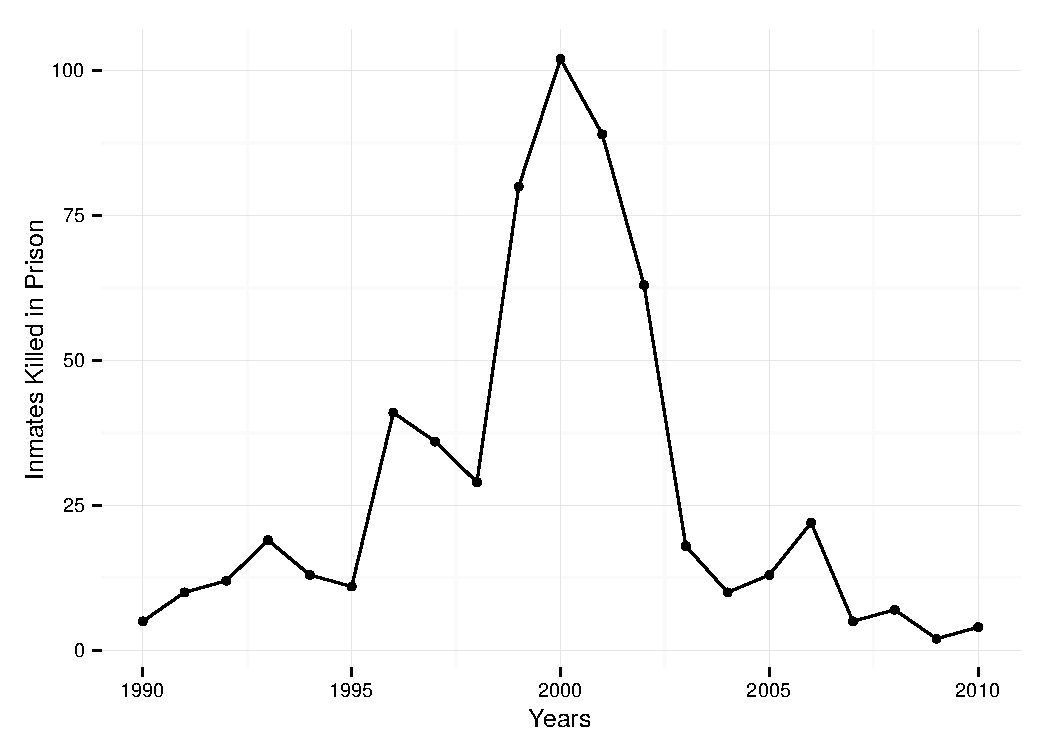
\includegraphics[height = 8cm, width = 1\linewidth]{gfx/fig5}
\caption[Inmates Killed in Prisons (1990--2010)]{Inmates Killed in Prisons (1990--2010)\footnotemark}
\label{fig:fig5}
\end{figure}
\end{center}

The\footnotetext{Source: Own authorship, with data provided by \citep[147]{dias2011pulverizaccao}.} rebellions in February 2001 were a major step in PCC's strategy of dominance. The \textit{Comando} unleashed simultaneous revolts in 29 prisons of the state, coordinating thousands of inmates. On the one hand, this series of attacks made it impossible for the government to deny the existence of the PCC, as it had done before. The rebellions were probable the largest ``publicity stunt'' for the group: at one blow, the PCC made itself both feared by the population and respected by criminals \citep[]{demedo2007}. Rumours go that just after the rebellion of 2001, there were long queues of prisoners asking to join the PCC ranks, and in Carandiru only, hundreds were baptised in a single gathering \citep[401]{dias2013organized}. The PCC had then entered into a virtuous circle: with new members, the \textit{Partido} was able to mobilise an even greater amount of financial and human resources, what would help them to control the remaining prisons in S\~{a}o Paulo. PCC's expansion to other regions was also intensified, and the cartel managed to extend its operations to other Brazilian states and even to other countries\footnote{The cartel has currently consolidated its presence in 22 of the 27 Brazilian states, has recently established itself in Paraguay and in Bolivia, earns about US\$ 60 million a year and plans to fund political campaigns in the next national elections to elect their own representatives \citep[apud][]{veja2013}.}. 

One of the tools that allowed the PCC to articulate such a powerful show of force was the widespread use of mobile phones within jails \citep[]{santos2010dimensao}. Brought by friends or relatives, mobile phones became a necessary tool for PCC members to organise themselves and coordinate actions outside prison walls. The 2001 rebellion started from the Carandiru prison, but it took only a few minutes for the inmates to spread the information to the other prisons via mobile phones \citep[]{terra2001rebeliao}. Although the government had been trying to ban cell phones from jails, corrupt agents still helped to smuggle such devices\footnote{Recently, it was reported that prison guards asked for about 10,000 dollars to smuggle a mobile phone into prison, around 30 minimum wages. See: \href{http://bit.ly/1rjtA3N}{http://bit.ly/1rjtA3N}. Access: 29th May, 2014.}.

As an indirect result of the rebellions in 2001, there was a remarkable change in the PCC's command. In 2001, the cartel was headed by Idemir Carlos Ambr\'{o}sio, nicknamed Sombra (``Shadow''), but no less than 5 months later, he was beaten to death in the same prison where the group had been founded. The leaders then became Gelei\~{a}o (``Big Jelly'') and Cesinha (``Little Ceasar''), two of the original members of the gang. Nevertheless, their rule did not last much longer. Although both criminals were responsible for articulating an important agreement with Rio de Janeiro's largest drug cartel -- the \textit{Comando Vermelho} -- their policies were considered ``too harsh'' to other PCC members, and they were suspected of using the group to increase their power at the expense of others. Moreover, Gelei\~{a}o and Cesinha were in solitary confinement, so it was difficult for them to oversee their subordinates and enforce their orders. The gangsters' wives (Petronilha and Aurinete) were to a large extent responsible for the \textit{Partido} \citep{istoe2013marcola}. 

In 2002, the two women started a feud to decide who would control the main businesses of the PCC. This event indirectly triggered the most significant change of the whole history of the group, when Marcos Willian Herbas Camacho (``Marcola'') become PCC's undisputed leader. Marcola has been the head of the organisation since 2002, and he is widely regarded as the person who modernised the PCC and turned it into the most feared and profitable drug gang in Brazil \citep[]{insight2012pcc}. According to news sources \citep{istoe2013marcola}, Ana Maria Olivatto, Marcola's ex-wife and lawyer, supposedly gave Cesinha's mobile phone number to the police, probably to help Marcola in one of the gang's internal disputes. A few weeks later, Aurinete, Cesinha's wife, killed Marcola's ex-wife. As a retaliation, Marcola gathered support from several PCC members who were unhappy with Gelei\~{a}o and Cesinha and decided to take control over the organisation. Accused of collaborating with the police and with a rival group, Cesinha was brutally murdered a couple of months later \citep[]{folha2006cesinha} and Gelei\~{a}o received a death sentence from the PCC \citep[]{congressoemfoco2006marcola}. Since the mid-2002, Gelei\~{a}o has been in solitary confinement because it is widely believed he will be killed as soon as he moves to a regular cell. With both leaders removed, Marcola was then put at the top of the organisation.

Marcola implemented several important measures just after he became PCC's \textit{capo di tutti capi}. Still in 2002, he decided to incorporate \textit{equality} into PCC's previous motto (``\textit{peace, justice and freedom}'') and dissolved the previous hierarchical structure that had been adopted by the gang since its foundation in 1993 \citep{biondi2010junto}. Consequently, all PCC members can now occupy any position in the organisation and no one -- with the partial exemption of the ``torres'' -- can force any \textit{irm\~{a}o} to do something against his will. Whenever possible, decisions are to be taken by consensus, and all political positions in the PCC are distributed according to the group's specific needs and the availability of ``technical group'' in the gang's ranks. In a certain sense, Marcola modernised the PCC by using the same techniques that nation-states employed to increase their efficiency: civil equality, the attack on privilege, and the creation of careers open to talent \citep[]{hobsbawm2010age}. Therefore, the PCC has become a rational, profit-driven enterprise, in which division of labour, productivity and loyalty to the firm are acknowledged and rewarded. 

This modernisation push can surely be credited to Marcola himself. Marcola is definitely not a regular inmate. An accomplished bank robber and a very skillful manager, Marcola has allegedly read more than 3,000 books since he was imprisoned in the 1990s, maintained a special taste for Nietzsche and Dostoevsky, and usually gives a copy of Sun Tzu's \textit{The Art of War} to every person he trusts \citep[]{epoca2005marcola}. 

Well-cultured and enjoying protection by the PCC itself in S\~{a}o Paulo's maximum security prison (Presidente Venceslau), Marcola has been administering the PCC's rise with great success. Recent footage shows that, using smuggled mobile phones, he closely oversees PCC's deals and alliances\footnote{``S\~{a}o Paulo under Attack'', a TV documentary made by Brazil's second largest broadcasting company (SBT) shows how easy it is for Marcola to pass orders to other PCC members. Link: \href{http://youtu.be/SOSDA-t1lOc}{http://youtu.be/SOSDA-t1lOc} (in Portuguese). Access: 30th May, 2014.}, and regularly discusses PCC's internal affairs with other high-level PCC members even while incarcerated.

\begin{center}
\begin{figure}[bth!]
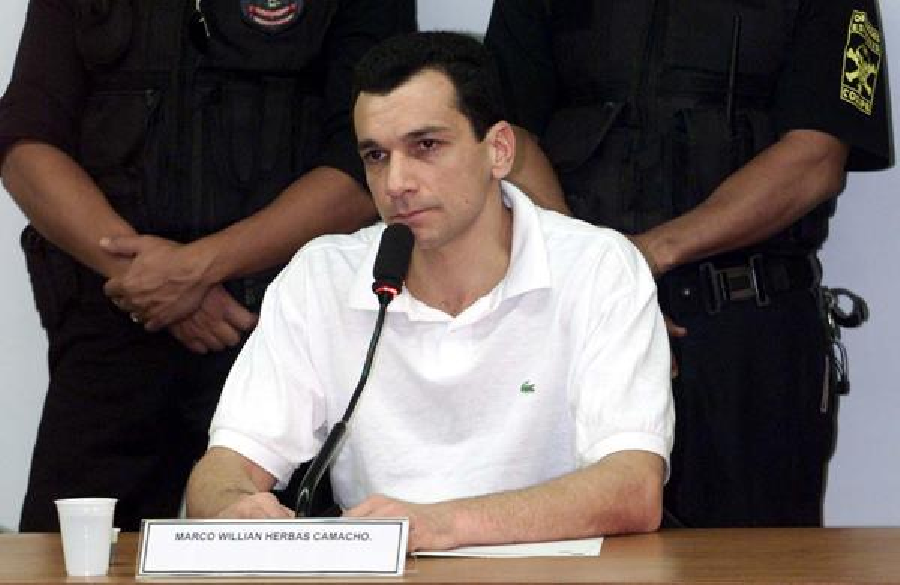
\includegraphics[height = 8cm, width = 1\linewidth]{gfx/fig6}
\caption[Marcola, PCC's leader]{Marcola, PCC's leader\footnotemark}
\label{fig:fig6}
\end{figure}
\end{center}

Marcola was also the mastermind behind the massive rebellions of 2006\footnotetext{Source: Cedoc/RAC.}. From March to July, he coordinated 82 rebellions in prisons in S\~{a}o Paulo and other neighbouring states. The PCC attacked hundreds of civilians, police officers, prison wardens and members of the government \citep[]{folha2006rebeliao, terra2008rebeliao}. It has recently been unveiled that the PCC even had a sophisticated plan to murder the current governor of S\~{a}o Paulo, Geraldo Alckmin, who has been taking a harsher stance against the criminal organisation \citep[]{estadao2013alckmin}. 

The group's terror tactics were ahighly effective against the population, too. During the attacks in May, 2006, schools and universities cancelled their classes, firms dismissed their employees, and all shopping malls were closed. Retail sales in S\~{a}o Paulo, Latin America's richest city, fell about 90\% in the week where most attacks were concentrated (12th t 17th May) \citep[]{uol2006pcc}. More importantly, about 500 people were killed -- including police officers, prison staff and civilians -- in just a few days, a very strong demonstration of force by any standard. From the PCC's viewpoint, the rebellion was a success: its impact was soon felt by the public and the government. For the first time in the group's history, there is plenty of evidence that the state accepted all PCC's demands and decided to go to the negotiation table with the gang. According to the International Human Rights Clinic, the cease-fire was conditional to the promise that the \textit{Tropa de Choque}\footnote{S\~{a}o Paulo's riot police.} would not enter into the penitentiaries, and the granting of additional rights to prisoners\footnote{Stable link: \href{http://bit.ly/1iK4h1i}{http://bit.ly/1iK4h1i}. Access: 2nd June, 2014.}. Two days after an informal meeting with Marcola (15th May 2006), the rebellions stopped \citep{folha2006fimataques}. 

\section{Hegemony: From 2006 to Date}

The attacks of 2006 represent the definitive step in PCC's consolidation process. The \textit{Partido} has successfully institutionalised its power, and to paraphrase the famous Weberian definition (\citeyear{weber1919politik}), the group has attained the monopoly of the legitimate use of physical force [\textit{Gewaltmonopol}] in the prison system. Furthermore, as predicted by theories of state formation, there has been a significant reduction in the number of prison rebellions. \autoref{fig:fig5} shows that the number of inmate deaths has also fallen drastically over the last years. Similarly, the use of symbolic violence, such as the beheading of members of other gangs, has virtually disappeared after 2006 \citep[166]{dias2011pulverizaccao}. 

PCC's monopolisation of violence has also brought changes to the the dynamics of violence in the city. According to several data sources, violence has decreased quickly in the poorest areas of S\~{a}o Paulo. \citet[]{de2010crime} indicates that the new ``crime courts'' deployed by the PCC in the outskirts of S\~{a}o Paulo are perhaps one of the central factors explaining the drop in homicide rates in city over the last two decade. Moreover, such courts could only be fully institutionalised after the PCC had ascended to the position of the legitimate legislative body among a minor, but relevant part of the residents of city suburbs.

We also note a shift in PCC's main financial sources. Whereas in the beginning of the 2000s the group obtained most of its funds via bank robberies and kidnapping, recently the \textit{Comando} has clearly become a drug cartel. It is not a coincidence that the group established itself as a powerful drug gang at the same time it consolidated its power over S\~{a}o Paulo's penal system. Drug dealing is clearly lucrative, but it also demands more bribes to police officers, a high investment on illegal weapons, and low levels of inter-gang violence to have a profitable business in the long. As pointed out by Alba Zaluar, drug traficking ``cannot last without institutional support''\footnote{Stable link: \href{http://bit.ly/1kguPwz}{http://bit.ly/1kguPwz}. Access: 2nd June, 2014.}. The graphs below show how the pattern of violence has changed in S\~{a}o Paulo\footnote{Source: Own authorship. Data provided by \citet[76]{dias2011pulverizaccao}}. 


\begin{center}
\begin{figure}[bth!]
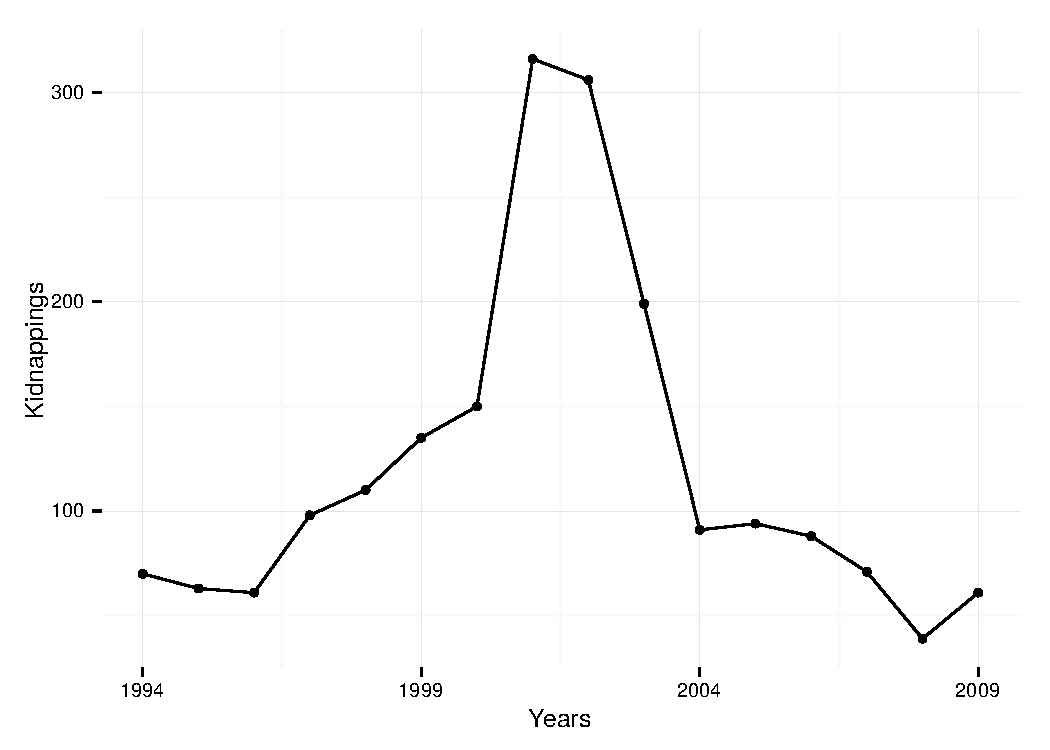
\includegraphics[height = 8cm, width = 1\linewidth]{gfx/fig7}
\caption[Kidnappings in S\~{a}o Paulo (1994--2009)]{Kidnappings in S\~{a}o Paulo (1994--2009)}
\label{fig:fig7}
\end{figure}
\end{center}

\newpage

\begin{center}
\begin{figure}[bth!]
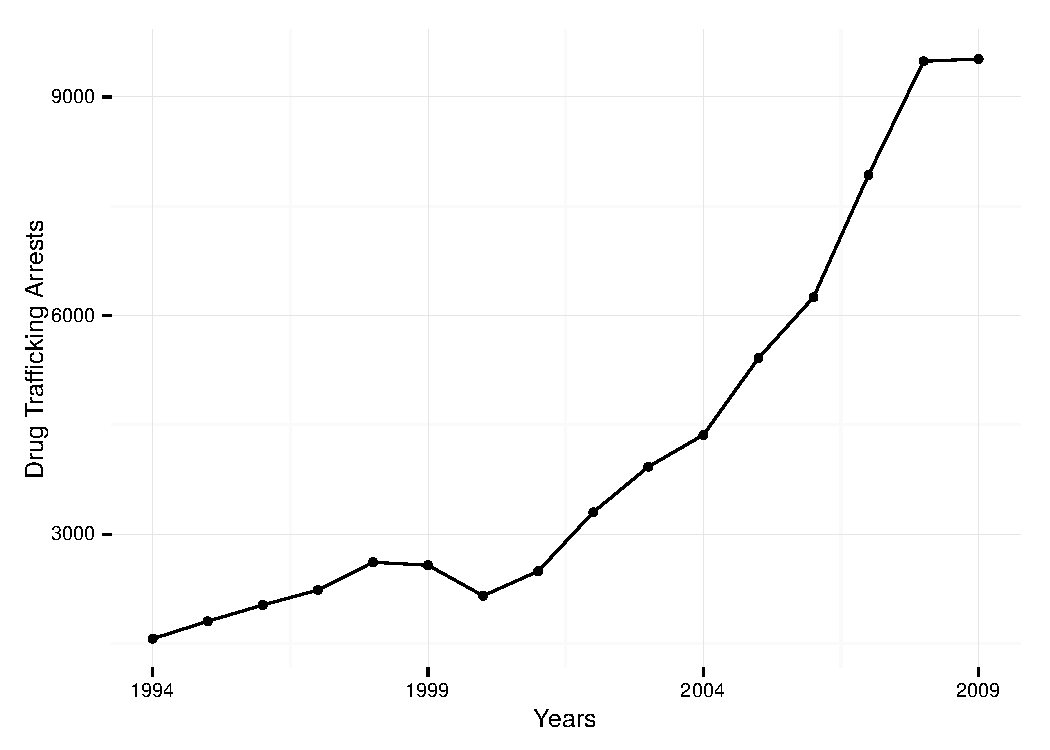
\includegraphics[height = 8cm, width = 1\linewidth]{gfx/fig8}
\caption[Drug Trafficking Arrests in S\~{a}o Paulo (1994--2009)]{Drug Trafficking Arrests in S\~{a}o Paulo (1994--2009)}
\label{fig:fig8}
\end{figure}
\end{center}


In a nutshell, the PCC has established itself as the largest prison gang in S\~{a}o Paulo by successfully devising a long-term strategy. In its initial stage, the group published a clear code of conduct that should be followed by all its members, and emphasised the need for financial support by punishing non-collaborative members to death. Later, the PCC promoted a spectacular demonstration of power that greatly impressed other inmates, the government and the public, therefore increasing their levels of credibility both inside and outside the prison system. During Marcola's leadership, the \textit{Comando} also modernised its practices by having a more inclusive discourse -- which stated that all prisoners should to treated equally -- and professionalised its cadres by adopting a meritocratic selection of members to its political positions. Finally, the PCC has skillfully used different types of threats and violence to eliminate rivals and improve collective action in the incarcerated population.

\section{Recruiting Potential Members}

The manner by which the PCC enlisted members has changed throughout its history. Whether in the beginning the gang used to selected its potential exclusively by their ties with the founding inmates, currently the procedure is much more professional and sophisticated. The first part is the \textit{batismo} (``baptism''). The baptism happens as follows. First, the inmate should already be a resident in a PCC-dominated prison, and show disposition to be engaged in the gang. As in any rationally-motivated enterprise, skillful prisoners are the ones that the PCC aspires to have in its ranks, and the cartel tries to choose only those who have already ``represented''\footnote{Here I tried to stick to the original term, \textit{representado} literally ``represented'', because it can also find an easy translation in English. To ``represent'' is also used with the same meaning in the United States, and the Urban Dictionary defines it as ``Go and be a good example to the others of your group or in your position''. This is precisely the idea conveyed by the PCC's native term. See: \href{http://www.urbandictionary.com/define.php?term=represent}{http://www.urbandictionary.com/define.php?term=represent}. Access:  12th June, 2014.} the criminal underworld in important situations \citep[99]{biondi2007relacoes}. Those detainees are called \textit{primos} (``cousins'') and are already closer to be admitted to the group. 

After this stage, there is what \citet[100]{biondi2007relacoes} aptly call the ``construction of the \textit{irm\~{a}o} (``brother''), how the PCC members are called. This period can last for several months, and it is both an opportunity for the ``cousin'' to show his criminal abilities and for the members to assess the candidate. If the ``cousin'' is deemed fit for the gang, two detainees who are already affiliated with the cartel formally accept him in the PCC. The prisoner can either accept or refuse the invitation.

However, there are costs for both sides if the inmate decides to join the group. The two detainees who invited the new member will be then considered his \textit{padrinhos} (``godfathers''), and should take some responsibility for the future actions of their proteg\'{e}e. Therefore, nominating someone who later makes a mistake is something criminals clearly want to avoid, as punishment can sometimes be harsh \citep[101]{biondi2007relacoes}. Second, the PCC is also in trouble if it accepts members who do not meet the group's high standas. Not only their lack of skills might put in risk the gang's operations -- and thus lead to strong repression by the state -- but bad members are also more likely to miscalculate the effects  of their actions and force the group to engage in unreasonable disputes, both with other gangs and within the PCC itself.


%After being \textit{batizados} (``baptised'') by the cartel\footnote{The baptism usually works like this: an inmate who is already in a PCC-dominated prison (called \textit{primo} -- ``cousin'') can become a full member of the PCC after being formally invited to join the gang by two other \textit{irm\~{a}os} (``brothers''), detainees who are already affiliated with the cartel. If the inmate decides to accept the offer, those two detainees who invited him will be then considered his \textit{padrinhos} (``godfathers'') and take responsibility for future actions of their proteg\'{e}e. Since the process implies costs for the two detainees, they tend to indicate an third inmate only after long periods of friendship. This explains why prisoners may stay as \textit{primos} for years before they are officially accepted in the PCC \citep[210]{biondi2007relacoes}.}, the inmates are called \textit{irm\~{a}os} (``brothers'') and can claim that they belong to the group. Criminals generally address each other as \textit{ladr\~{a}o} (``thief'') regardless of the crime perpetrated by the individual, and although PCC members also use \textit{irm\~{a}os} to refer to each other, the more general term ``thief'' is employed very often. Its meaning, if derogatory, neutral or even complimentary, depends widely on context \citep[]{marques2009crime}. In contrast, police officers, members of rival gangs, and other enemies are called \textit{coisa} (``thing'') or \textit{verme} (``worm'') \citep[169]{dias2011pulverizaccao}. 

%There are three ``political positions'' that a PCC member can occupy, namely \textit{faxinas} (``cleaners''), \textit{pilotos} (``pilots''), and \textit{torres} (``towers'') \citep[110-123]{biondi2010junto}. The first group comprises inmates who work as mediators between prisoners and state institutions, and are also in charge of the cleaning and management of everyday affairs. \textit{Pilotos} are ``spokespeople'' to the inmates, and are democratically elected by the detainees to voice their concerns and represent them in negotiations \citep[1102]{dullo2012biondi}. ``Pilots'' are elected at many different levels, being usually a representatives of the cell, corridor and prison. The role of the \textit{torres} is a bit more difficult to grasp. From what is currently known, the towers are groups of senior inmates who jointly debate and decide (usually by consensus) some of the most serious issues regarding the organisation, such as giving order, solving disputes and ordering punishments. However, PCC members are quite elusive about the meaning and scope of such groups, and so far there is not a single academic research that clarifies under what circunstances the torres are called to act and what tasks they are allowed to perform \citep{biondi2010junto}.

In this sense, two questions remain unanswered. Firstly, if the PCC has managed to control most of the jails in S\~{a}o Paulo, why does not \textit{every inmate} want to be a member of the gang? While it is known that the PCC has a relatively strict admission process, where a new member can only join the group after being nominated by two members, there are many prisoners who do not even \textit{want} to be part of the \textit{Comando}. It has been estimated that 
\textit{less then 3\%} of the inmates in S\~{a}o Paulo have any formal relationship with the PCC\footnote{Although the number seems small, the cartel has about 8,000 members. In comparison, the Mexican Mafia, the biggest prison organisation in the United States, has 150--300 official members \citep[703]{skarbek2011governance}. Thus, the PCC is 53 times larger than \textit{La Eme}  if we use the most conservative estimate.} \citep[]{bbc2013pcc, veja2013crescimentopcc}. \citep[98]{biondi2007relacoes} notes that in provisory detention facilities the number is even smaller, about 1\%. Why are the remaining prisoners not engaged in joining the cartel, if they could have some clear benefits? As far as I know, this large share of the incarcerated population has not been the object of any qualitative study, let alone a model formulation. Would joining the PCC be a dominant strategy, or does an ``independent'' position in a gang-dominated prison also have some benefits?

Another puzzling question is how the PCC manages to select skillful criminals in an environment marked by uncertainty. Lack of trust is also widespread amongst criminals, it is difficult to establish a credible commitment of both parts, non-members and the PCC. Choosing a good member is a much more difficult task for a prison gang than it is for the government or for a firm, since a bad decision can literally be deadly to the the group. Thus, how has the PCC succeeded in choosing its members quite successfully so far?

% Communication in prisons is notably limited, so inmates have strong incentives to fake their credentials, show a different behaviour and try to obtain advantages at the group's expense. 

The next chapters aim to answer those questions. In the following section I develop a simple game-theoretical model to address the issues of individual choice in a PCC-dominating correctional facility. In \autoref{ch:chap5} I use agent-based computational modeling to evaluate the different uses of violence by prison gangs. The model is informed by qualitative data gathered by scholars, as discussed in \hyperlink{page.17}{chapter 2}, and could in theory be generalised and be tested in similar environments. In this sense, my goal here is to formulate two simple, intuitive models that expand the current findings on one of the world's largest prison gangs and provide subsidies for a future general theory of gang violence.

%This is largely in line with theories of state formation. For instance, \citet{buchanan1973defense} argues that a monopoly of violence is better than a free market competition on protection since the monopolist has strong incentives to under-produce violence and allocate those resources elsewhere\footnote{Theoretically, one can say that the underproduction of violence is Pareto superior in a partial equilibrium setting.} The author writes that after a monopoly has been established ``[\dots] resources involved in enforcement may be freed for the  production of alternative goods and services that are positively valued; the taxpayer has additional funds that he may spend on alternative publicly provided or privately marketed goods and services'' \citep[402]{buchanan1973defense}. Those resources have been mainly invested in the enlargement of the group's stake in the drug selling business in S\~{a}o Paulo, and as we have show in \autoref{fig:fig8}, it seems that such strategy has been largely successful.

